% !TeX spellcheck = english
% !TEX root = thesis.tex
\section{Experimental Results}
    \subsection{Fabrication of Crystalline Silicon Nanoparticles}
        \label{sec:Fabrication}

        \subsubsection{Laser Writing of Nanoparticles}

            \begin{figure}[!ht]
                    \begin{center}
                        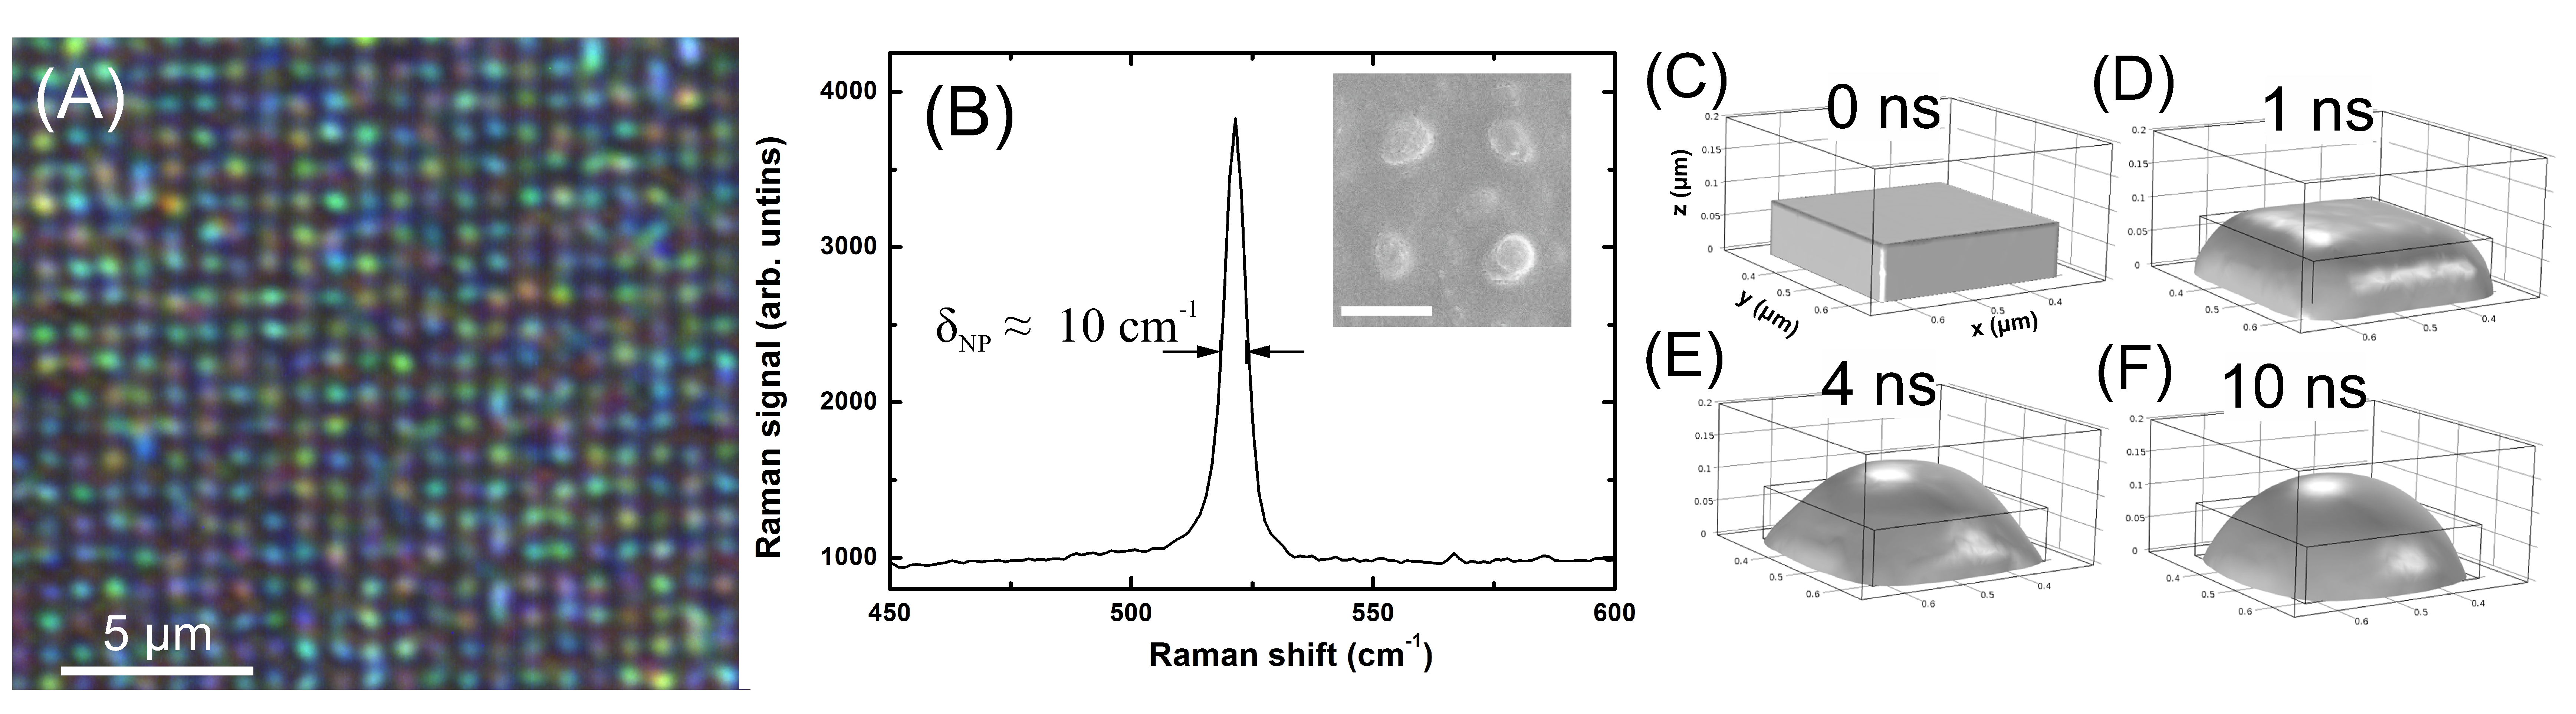
\includegraphics[width=0.9\textwidth]{figs/results/fab/LaserWriting.eps}
                    \end{center}
                    \caption{}
                    \label{fig:LaserWriting}
            \end{figure}

            Under the optimal conditions of fabrication, the method described in Sec. \ref{met:writing} creates an array of nanoparticles with a period of about 0.9~$\mu$m,
            exhibiting bright colors, caused by resonant scattering (Fig.~\ref{fig:LaserWriting}A). Though the cutting should
            produce an array of square patches, SEM images show that the nanoparticles look almost circular from the top
            (Fig.~\ref{fig:LaserWriting}B). This is due to the fact that thermal isolation of the patch from the rest of the film causes it to overheat
            during the cutting process and dewet into spherical nanoparticles. In order to provide deeper insight into the patches reshaping mechanism,
            the time dynamics of a square liquid silicon patch with a height of 80~nm and side of 300~nm
            (Figs.~\ref{fig:LaserWriting}C) on top of a fused silica substrate were modeled in COMSOL software, solving the incompressible Navier-Stokes
            equations and taking into account the parameters of the used materials. The modeling shows that after ten nanoseconds
            the patch is transformed into a hemisphere with a height of 140~nm and width of 350~nm (Figs.~\ref{fig:LaserWriting}C-F),
            which is in qualitative agreement with the experimentally observed shapes.

            The corresponding Raman signals from these nanoparticles also reveal the crystalline state of the nanoparticles written
            by the laser, demonstrating a narrow peak at 520~cm$^{-1}$, with a half-width of about 10~cm$^{-1}$ (Fig.~\ref{fig:LaserWriting}B).
            This half-width corresponds to mean crystallite size of less than 10~nm, according to previous studies~\cite{campbell1986effects}.

        \subsubsection{Laser Transfer of Nanoparticles}
            \begin{figure}[!ht]
                    \begin{center}
                        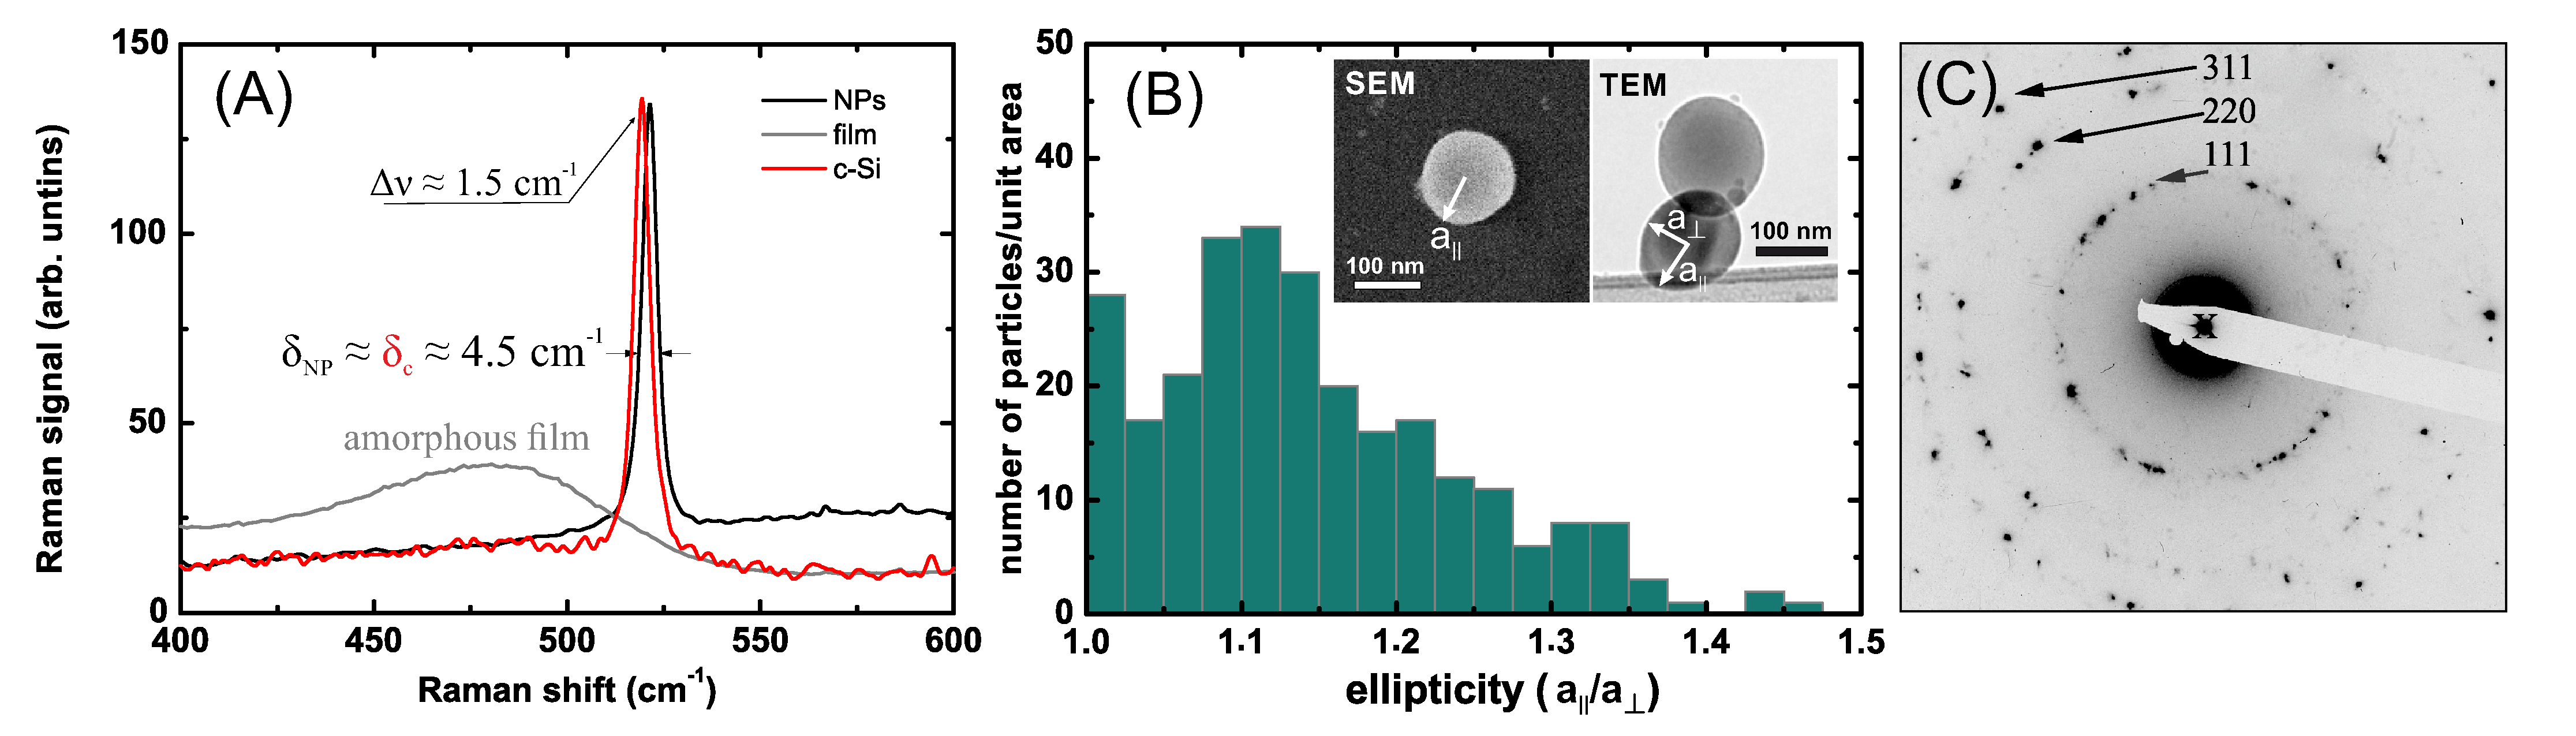
\includegraphics[width=0.9\textwidth]{figs/results/fab/Crystallinity.eps}
                    \end{center}
                    \caption{}
                    \label{fig:Crystallinity}
            \end{figure}

                The initial a-Si:H film, from which the particles were fabricated was amorphous, which was supported by its broad Raman
            peak, centered around 480~cm$^{-1}$. The measured Raman spectra from individual nanoparticles fabricated using the method
            described in Sec. \ref{met:transfer} had narrow peaks at 521.5~cm$^{-1}$, corresponding to the crystalline cubic diamond structure.
            The reference Raman signal from a bulk crystalline silicon wafer and the literature data say that the Raman peak of pure crystal
            corresponds to 520~cm$^{-1}$.
            The slight positive shift of the peak of the nanoparticles $\Delta$$\nu$ = 1.5~cm$^{-1}$ can be explained by the
            residual compressive stress~\cite{de1996micro} in the nanoparticles. Another important characteristic extracted from the Raman spectra
            was the crystallite size, which is larger than $\sim$20~nm, because the Raman peaks of the nanoparticles have
            almost the same half-width (4--5~cm$^{-1}$) as the peak from bulk crystalline silicon wafer (4.5~cm$^{-1}$)
            ~\cite{campbell1986effects}.

                The Raman measurements agree with characterization of the printed nanoparticles by means of transmission electron
            microscopy (TEM). Specimen grids (3-mm-diameter, 200-mesh copper grids, coated on one side with a 20-nm-thick
            film of amorphous carbon) were used to collect nanoparticles ablated from the a-Si:H film. The size, structure, and composition
            of the collected nanoparticles were determined using bright and dark field TEM imaging, see the inset in Fig.
            ~\ref{fig:Crystallinity}B. The analysis of the electron diffraction pattern from several nanoparticles shows clear maxima,
            corresponding to certain crystalline planes (Fig.~\ref{fig:Crystallinity}C). Because the specimen grids were uneven, the
            nanoparticles were deposited at different angles to the substrate meaning that TEM imaging also provides information
            on the oblateness of the particles along the direction perpendicular to the substrate surface, giving the average
            ellipticity about $a_{\parallel}/a_{\perp}\approx$1.12, where $a_{\parallel}$($a_{\perp}$) is the particle semi-major
            (semi-minor) axis oriented parallel (perpendicular) to the surface of the substrate. Scanning electron
            microscopy (SEM, Carl Zeiss, Neon 40) confirmed that the particles possess axial symmetry along the substrate
            normal (Fig.~\ref{fig:Crystallinity}B). These results correlate with previously observed oblateness of the printed silicon
            nanoparticles~\cite{zywietz2014laser}.

                According to previous~\cite{zywietz2014laser, zywietz2014generation}, the mean size of the printed nanoparticles
            strongly depends on laser fluence. In the experiments similar behavior was also observed. Two different
            regimes of the nanoparticle generation were observed. In the first regime, the nanoparticle size increases
            with an increase of fluence up to 150~mJ/cm$^{2}$, manifesting in the change of their colors from blue to red
            (Figs.~\ref{fig:Darkfield}A--C). Such behavior can be described in terms of the spallation mechanism of laser ablation, where
            a thin molten layer is spalled due to the laser-induced tensile pressure waves~\cite{ionin2013thermal,wu2014microscopic},
            breaking into a number of liquid droplets via the Rayleigh-Plateau instability~\cite{papageorgiou1995breakup}.
            The photomechanically spalled volume increases as V$\sim$ln(E) under the action of a Gaussian beam, owing to the
            logarithmic dependence of the spalled surface layer area r$^{2}$$_{s}$$\sim$ln(E)~\cite{bauerle2013laser}, whereas
            the thickness of the layer remains almost constant~\cite{ionin2013thermal} or even decreases~\cite{wu2014microscopic}.
            In previous studies of nanoparticle frabrication from crystalline silicon such an increase of the molten volume led
            to an increase in the number of nanoparticles~\cite{zywietz2014generation} and their size~\cite{zywietz2014laser},
            which agrees with the current results (Fig.~\ref{fig:Darkfield}A--C).

                The second regime of the nanoparticle fabrication corresponds to flucencies F~$>$~150~mJ/cm$^{2}$, where large (red) nanoparticles
            are created alongside small nanoparticles with a much broader size distribution (Fig.~\ref{fig:Darkfield}D). This regime is related to
            unstable boiling of superheated silicon~\cite{bulgakova2001pulsed, ionin2013thermal, wu2014microscopic}, when the
            nanoparticle formation occurs through explosive decomposition of the material into vapor and small
            clusters/droplets~\cite{itina2009molecular,wu2014microscopic}, yielding nanoparticles with the mean sizes smaller than
            100~nm~\cite{amoruso2004generation}. Small silicon nanoparticle fabrication in this regime has been extensively studied
            over the last two decades~\cite{amoruso2004generation, tull2006formation} for a number of biomedical applications.
            However, one can conclude that the high-fluence regime (Fig.~\ref{fig:Darkfield}D) is not desirable for reproducible Mie-type
            nanoresonators fabrication, whereas the low-fluence regimes (Fig.~\ref{fig:Darkfield}A--C) provide much more controllable
            nanoparticle fabrication and deposition. The Raman, TEM and SEM characterization of the printed silicon nanoparticles
            helped to determine their almost perfect crystalline phase, meaning that it is possible to fabricate the crystalline
            silicon nanoresonators from amorphous films, which is very useful for low-loss all-dielectric nanophotonics.

    \subsection{Characterization of Resonant Optical Modes of the Nanoparticles}
        \label{sec:DarkfieldExp}

        \begin{figure}[!ht]
                \begin{center}
                    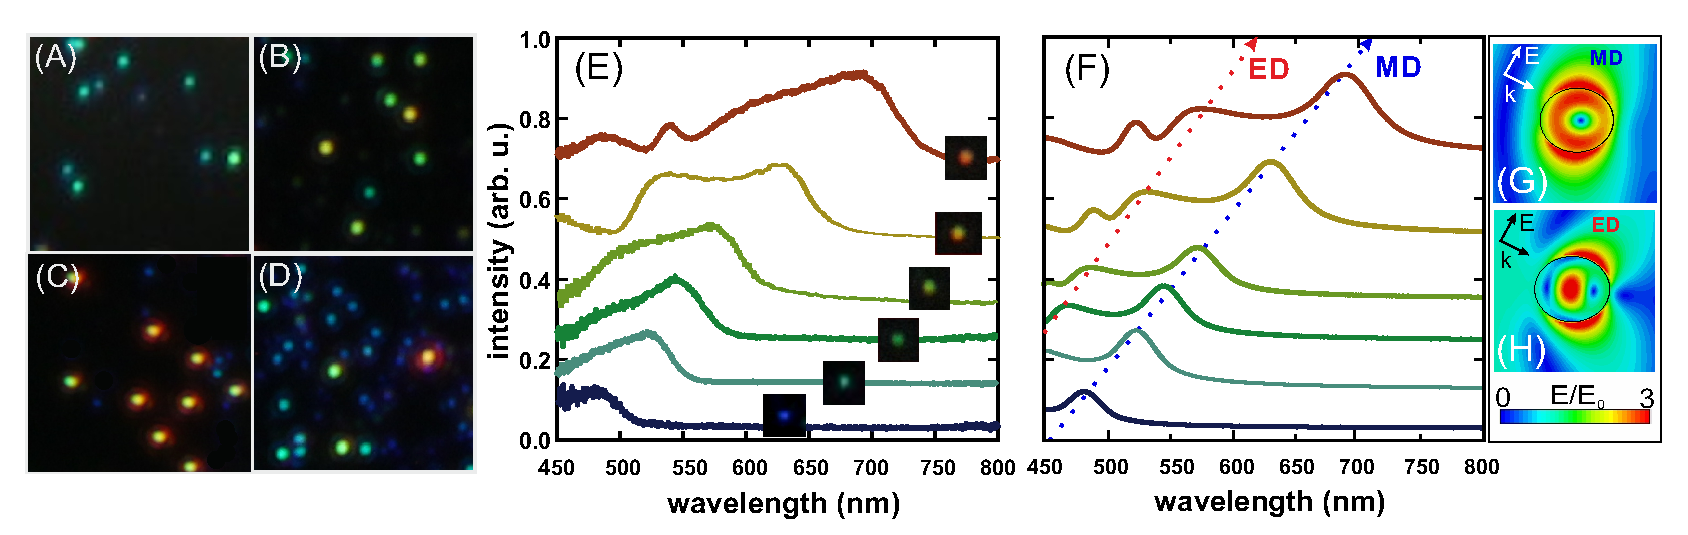
\includegraphics[width=0.9\textwidth]{figs/results/char/DarkField.eps}
                \end{center}
                \caption{Dark-field optical images of silicon nanoparticles fabricated at different peak fluencies:
                120 (A), 130 (B), 140 (C), 160~mJ/cm$^{2}$ (D). Experimental (E) and theoretical (F) spectra for
                scattered p-polarized incident light (angle of incidence is 65$^{\circ}$) from individual nanoparticles
                with the radius parallel to substrate surface a$_{\parallel}$ = 55~nm (blue), 65~nm (spring green),
                68~nm (green), 72~nm (olive), 85~nm (yellow) and 92~nm (red) with the ellipticity coefficient of 1.12.
                Numerically calculated electric field distributions in the silicon nanoparticle with a$_{\perp}$ = 85~nm
                 the wavelengths of 635~nm (G) and 525~nm (H).}
                \label{fig:Darkfield}
        \end{figure}

            Dark field scattering measurements showed that the nanoparticles posses a number of resonances, corresponding to different
        Mie-type resonances, see Fig. \ref{fig:Darkfield}. To determine which resonances correspond to electric dipole (ED) and
        magnetic dipole (MD) resonances, the scattering properties of and electric field distribution near the nanoaparticles were
        modeling using the FIT technique in CST Microwave Studio.

            The scattering geometry was modeled as a c-Si ellipsoid with different axis
        ($a_{\perp}$ and $a_{||}$) and the fixed ellipticity $a_{\parallel}/a_{\perp}\approx$~1.12, i.e. for
        the most probable ellipticity parameter in the experiments. The ellipsoid was irradiated by a plane wave
        at the angle 65$^{\circ}$ in vacuum. The optical properties for
        c-Si were taken from Ref.~\cite{vuye1993temperature}. Modeling of scattering spectra (Fig.~\ref{fig:Darkfield}F) showed good agreement
        with the corresponding experimental ones (Fig.~\ref{fig:Darkfield}E), whereas the modeled electric field distributions
        in the ellipsoids at different wavelengths proved the excitation of MD (Fig.~\ref{fig:Darkfield}G) and ED (Fig.~\ref{fig:Darkfield}H).

    \subsection{Determining Size of Nanoparticle from Optical Resonance Positions}

        \begin{figure}[!ht]
                \begin{center}
                    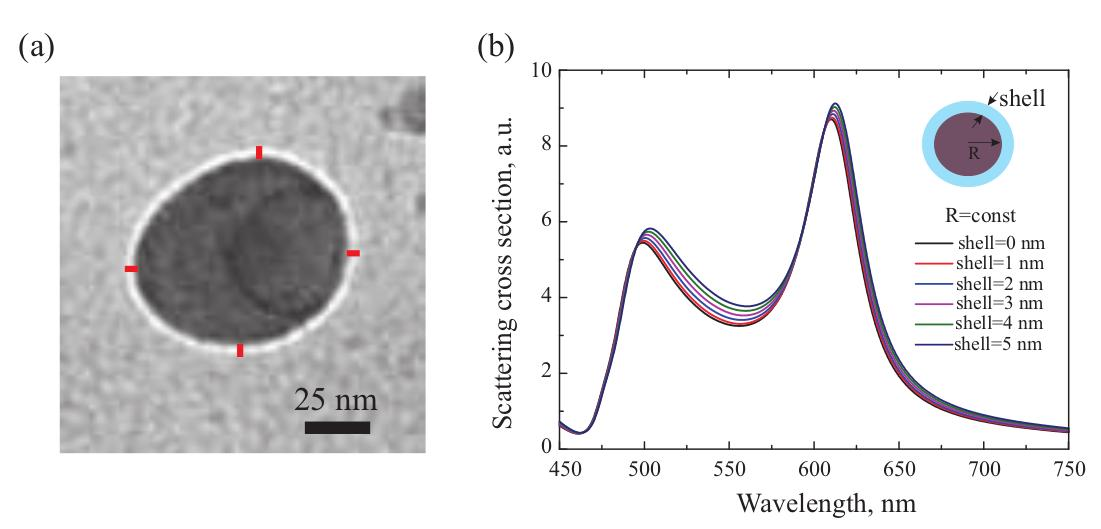
\includegraphics[width=0.9\textwidth]{figs/results/char/CoreShell.jpg}
                \end{center}
                \caption{\textbf{a}. TEM image of the typical silicon nanoparticle fabricated using laser-induced
                            forward transfer technique. Red lines represent 5 nm. \textbf{b}. Total scattering cross sections of
                            silicon nanoparticle (R = 75 nm) coated with silica layers with different thicknesses.}
                \label{fig:CoreShell}
        \end{figure}

        Resonant optical properties of silicon nanoparticles are known to be sensitive to their shape\cite{zywietz2015electromagnetic},
        crystallinity\cite{zywietz2015electromagnetic, dmitriev2016laser}, to the substrate\cite{miroshnichenko2015substrate} and
        to the thickness of native oxide layer\cite{zywietz2015electromagnetic, fu2012directional},
        which is always present on silicon surface\cite{morita1990growth}. In this work, the shape of the particles has been controlled using
        SEM measurements, while the diameter of silicon core has been extracted from dark-field spectroscopy experiments.
        In order to analyze the influence of native silicon oxide layer on the optical properties of the studied nanoparticles,
        additional experimental measurements and numerical simulations were done. The typical thickness of the native oxide layer was
        estimated by transmission electron microscopy (TEM) of a typical silicon nanoparticle using, see Fig. \ref{fig:CoreShell}A.
        The measurements showed that nanoparticles are coated with a silica layer, at most 5-nm-thick, which is in good agreement
        with previously reported results\cite{zywietz2015electromagnetic, fu2012directional}. To analyze the influence of the oxide
        layer on the resonant properties of nanoparticles,
        total scattering cross section spectra of a crystalline silicon nanoparticle (D = 150 nm) surrounded by
        silica shells with different thicknesses were simulated, see Fig. \ref{fig:CoreShell}. For the sake of simplicity, the simulations have been carried out
        using Mie theory\cite{bohren1983absorption}. The results of the simulations confirm that in the case of a fixed silicon core diameter, the appearance of an additional
        5-nm-thick silica layer leads to red spectral shifts of both electric and magnetic dipole resonances of the
        nanoparticle at most by $≈ 4.2$nm and $≈ 2.5$nm. The influence of different substrates has been analyzed in
        Ref. \cite{miroshnichenko2015substrate} The authors have demonstrated that both electric and magnetic dipole resonances of
        crystalline silicon nanoparticle
        placed on the fused silica substrate exhibit small red spectral shifts with respect to the resonances of the nanoparticle
        in free space. In the case of nanoparticle with the diameter of $D = 130 $nm these shifts are around $≈ 3.5 $nm and $≈ 0.5$ nm.
        Therefore, the spectral shift of the nanoparticle’s magnetic dipole resonance is almost insensitive to both
        the substrate and the native silica layer. This allows for accurate estimation of the the diameter of silicon core of the nanoparticle
        from the spectral position of magnetic dipole resonance in the dark-field spectroscopy measurements by
        comparing to the simulations based on Mie theory.


    \subsection{Raman Scattering Enhancement from Single Nanoparticles}
        \label{sec:RamanExp}
        Theoretically predicted enhancement of Raman scattering at different Mie-resonances (see Sec. \ref{sec:Theory}) was directly compared with to
        experiments with individual crystalline silicon (c-Si) nanoparticles on a fused silica substrate.

        \begin{figure}[!ht]
            \begin{center}
                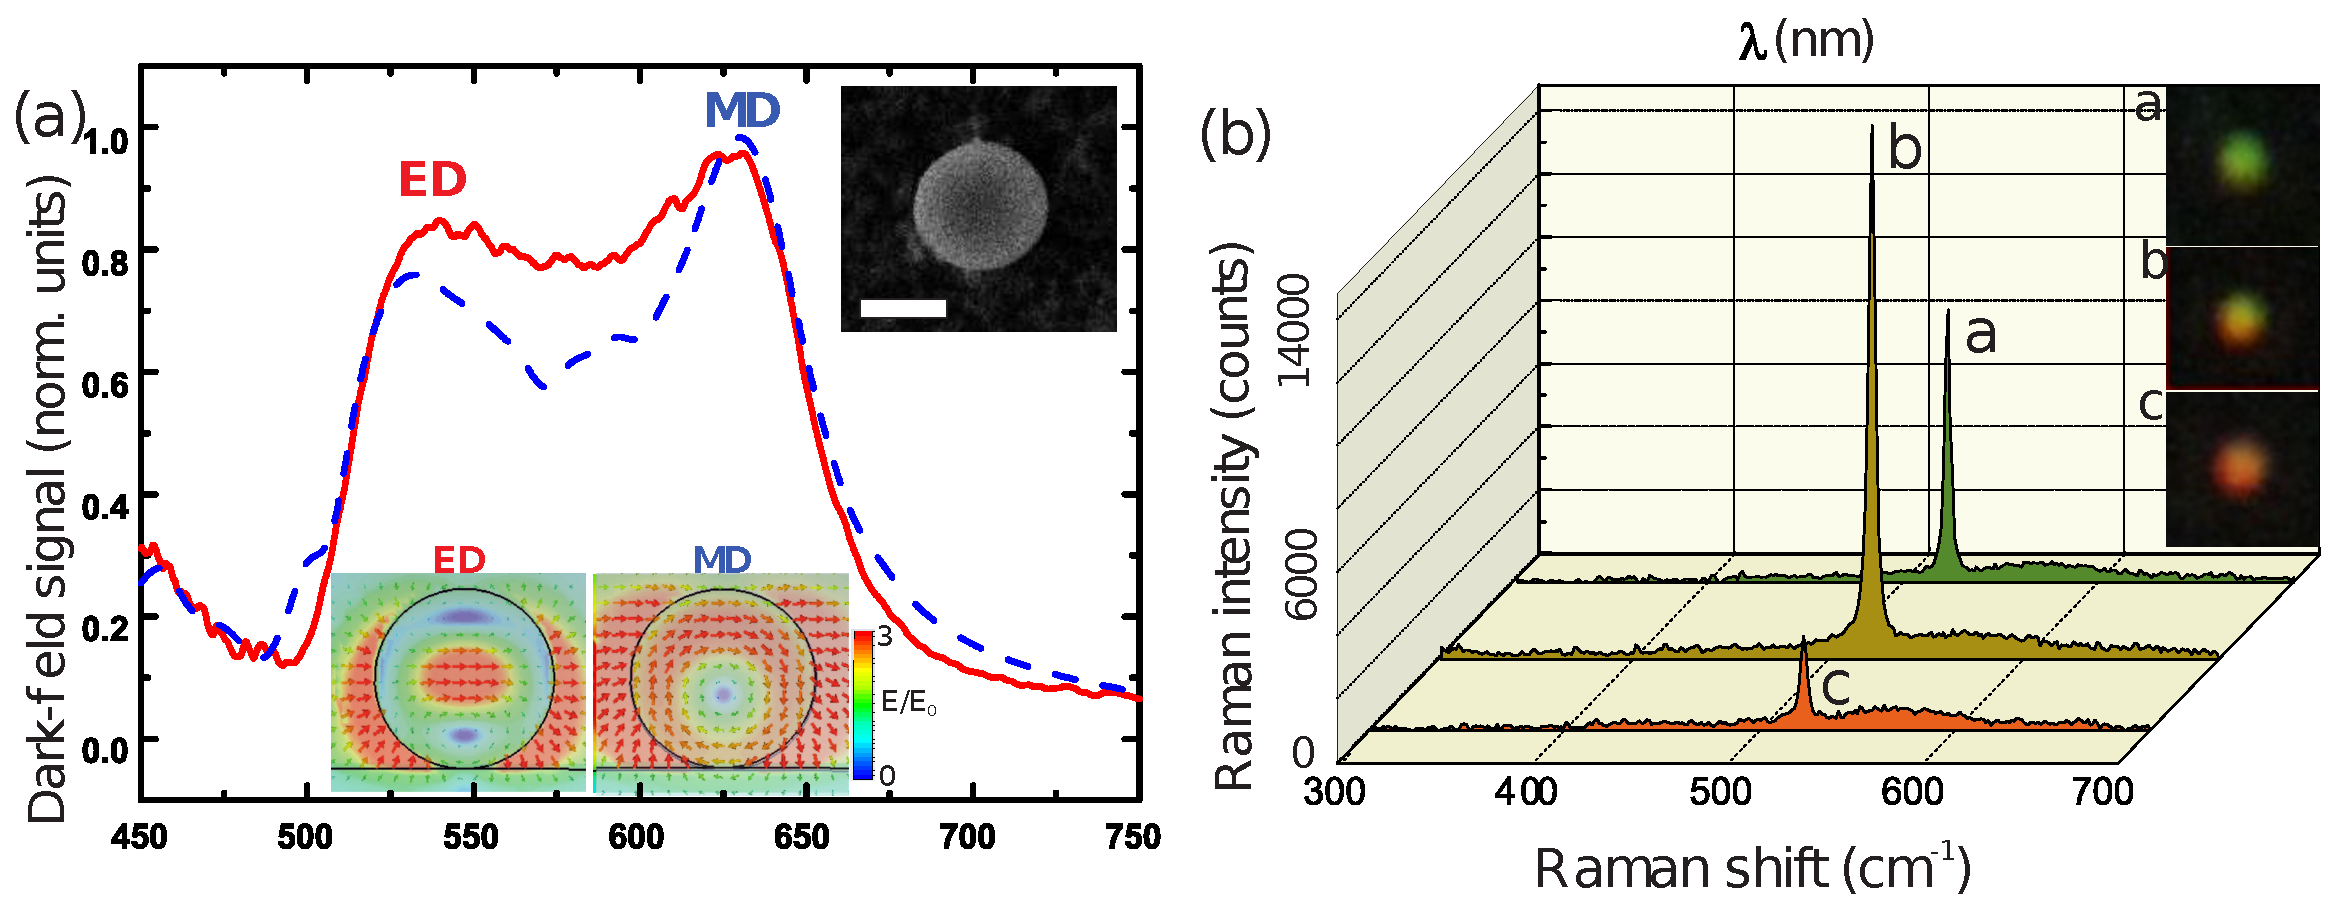
\includegraphics[width=0.9\textwidth]{figs/results/enhance/EnhancementExperiment.eps}
            \end{center}
            \caption{(\textbf{a}) Experimental (solid) and theoretical (dashed) scattering spectra for s-polarized incident light.
            Bottom inset: the electric field distribution at different wavelengths, corresponding to electric dipole (ED) and magnetic
            dipole (MD) resonances. Upper inset: SEM image of typical ablative c-Si nanoparticle (scale bar represents 100~nm). (\textbf{b})
            Raman spectra for different nanoparticles at the excitation wavelength of 633 nm and the corresponding dark-field optical images of the
            nanoparticles: (a) D=153 nm, (b) D=158 nm, (c) D=173 nm.}
            \label{fig:EnhancementExp}
        \end{figure}

        The measured Raman scattering signal from individual nanoparticles exhibits extremely strong dependence on their size
        and color in the dark-field images (Fig.~\ref{fig:EnhancementExp}b). Such a dependence for the excitation light at the wavelength
        $\lambda$=633~nm shows a maximum of Raman scattering for nanoparticles with $D\approx 155$~nm, supporting MD resonance
        at this wavelength. The maximum value of the enhancement factor (EF) for nanoparticles with MD in comparison with
        nanoparticles with diameters $D\approx125$~nm and $D\approx175$~nm is about $EF\approx$140. The calculation of EF
        from experimental data is based on the formula: EF~=~(I/I$_{\rm norm}$)$\times$(V/V$_{\rm norm}$), where I is Raman
        scattering signal from a studied nanoparticle with known diameter and volume V, I$_{\rm norm}$ is Raman signal from
        a nanoparticle of known volume V$_{\rm norm}$ with the smallest observed signal. To make such a normalization, the
        nanoparticle with $D\approx$135~nm was chosen.
        In order to distinguish contributions from each type of Mie resonances, the generalized EF dependence of Raman
        scattering should be represented in terms of the dimensionless nanoparticle diameter $D/\lambda_{\rm Si}$,
        taking into account different refractive indices at different wavelengths (Fig.~\ref{fig:EnhancementExpTheory}). Such a dependence
        exhibits a pronounced maximum with a peak $EF\approx$140 at D/$\lambda_{\rm Si}$ $\approx$ 1, i.e. near the
        magnetic dipole resonance. This value is 5-7 times larger than EF for the electric dipole. Insets in Fig.~\ref{fig:EnhancementExp}a
        provide an illustrative interpretation of this enhancement. At the MD resonance, a larger fraction of electromagnetic
        energy is stored inside the nanoparticle, thus increasing total Raman polarization and emission.
        Corresponding theoretical calculations for perfect spherical c-Si nanoparticles predict even larger difference between
        MD and ED ($\sim$ 10), which is not perfectly matched with the observed results owing to the existence of nanoscale
        deviations and a thin natural oxide layer~\cite{fu2012directional, zywietz2015electromagnetic}. Nevertheless, the
        Raman signal enhancement in the vicinity of MD is in excellent agreement with the analytical model from Sec. \ref{sec:Theory}.
        The data shown in Fig.~\ref{fig:EnhancementExpTheory} is limited to nanoparticle diameters $D/\lambda_{\rm Si}<1.3$ as the fabrication method
        does not allow to make larger particles without pronounced ellipticity. At the same time, even small deviation from the spherical shape leads to
        suppression of the MQ resonance~\cite{fu2012directional}, limiting experimental demonstrations of the enhancement to MD and ED resonances.

        \begin{figure}[!hb]
            \begin{center}
                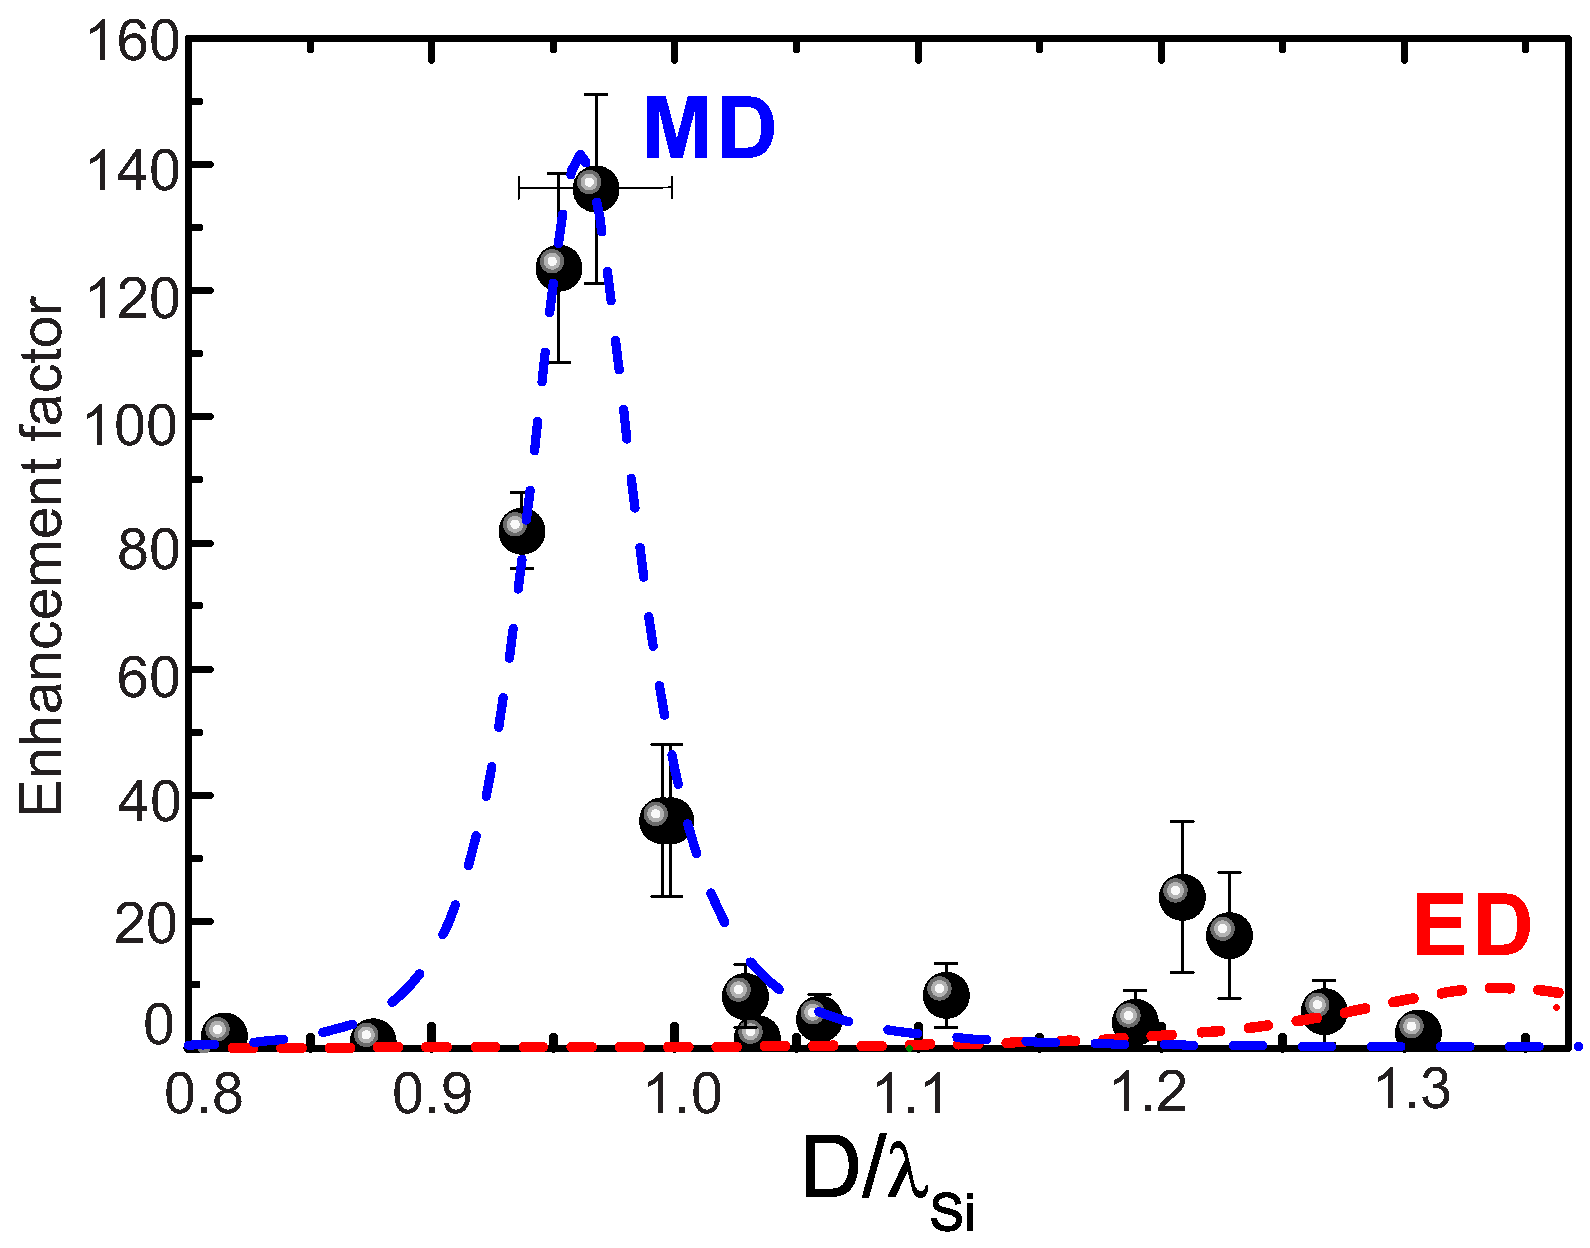
\includegraphics[width=0.5\textwidth]{figs/results/enhance/EnhancementExperimentTheory.eps}
            \end{center}
            \caption{Theoretical (dashed curves) and experimental (black dots) dependencies of the enhancement factor for Raman
            scattering from spherical silicon nanoparticles on their diameter D normalized to the excitation wavelength in silicon.
            Theoretical dependence consists of two contributions from magnetic dipole (blue dashed curve) and electric dipole
            (red dashed curve).}
            \label{fig:EnhancementExpTheory}
        \end{figure}
